\documentclass[11pt, a4paper]{article}
\usepackage{pdfpages}
\usepackage{parallel}
\usepackage[T2A]{fontenc}
\usepackage{ucs}
\usepackage[utf8x]{inputenc}
\usepackage[polish,english,russian]{babel}
\usepackage{hyperref}
\usepackage{rotating}
\usepackage[inner=2cm,top=1.8cm,outer=2cm,bottom=2.3cm,nohead]{geometry}
\usepackage{listings}
\usepackage{graphicx}
\usepackage{wrapfig}
\usepackage{longtable}
\usepackage{indentfirst}
\usepackage{array}
\usepackage{tikzsymbols}
\usepackage{soul}
\usepackage[ruled,vlined]{algorithm2e}
%\counterwithout{figure}{section} 

\usepackage{url}
\makeatletter
\g@addto@macro{\UrlBreaks}{\UrlOrds}
\makeatother

\newcolumntype{P}[1]{>{\raggedright\arraybackslash}p{#1}}
\frenchspacing
\usepackage{fixltx2e} %text sub- and superscripts
\usepackage{icomma} % коскі ў матэматычным рэжыме
\PreloadUnicodePage{4}

\newcommand{\longpage}{\enlargethispage{\baselineskip}}
\newcommand{\shortpage}{\enlargethispage{-\baselineskip}}

\def\switchlang#1{\expandafter\csname switchlang#1\endcsname}
\def\switchlangbe{
\let\saverefname=\refname%
\def\refname{Літаратура}%
\def\figurename{Іл.}%
}
\def\switchlangen{
\let\saverefname=\refname%
\def\refname{References}%
\def\figurename{Fig.}%
}
\def\switchlangru{
\let\saverefname=\refname%
\let\savefigurename=\figurename%
\def\refname{Литература}%
\def\figurename{Рис.}%
}

\hyphenation{admi-ni-stra-tive}
\hyphenation{ex-pe-ri-ence}
\hyphenation{fle-xi-bi-li-ty}
\hyphenation{Py-thon}
\hyphenation{ma-the-ma-ti-cal}
\hyphenation{re-ported}
\hyphenation{imp-le-menta-tions}
\hyphenation{pro-vides}
\hyphenation{en-gi-neering}
\hyphenation{com-pa-ti-bi-li-ty}
\hyphenation{im-pos-sible}
\hyphenation{desk-top}
\hyphenation{elec-tro-nic}
\hyphenation{com-pa-ny}
\hyphenation{de-ve-lop-ment}
\hyphenation{de-ve-loping}
\hyphenation{de-ve-lop}
\hyphenation{da-ta-ba-se}
\hyphenation{plat-forms}
\hyphenation{or-ga-ni-za-tion}
\hyphenation{pro-gramming}
\hyphenation{in-stru-ments}
\hyphenation{Li-nux}
\hyphenation{sour-ce}
\hyphenation{en-vi-ron-ment}
\hyphenation{Te-le-pathy}
\hyphenation{Li-nux-ov-ka}
\hyphenation{Open-BSD}
\hyphenation{Free-BSD}
\hyphenation{men-ti-on-ed}
\hyphenation{app-li-ca-tion}

\def\progref!#1!{\texttt{#1}}
\renewcommand{\arraystretch}{2} %Іначай формулы ў матрыцы зліпаюцца з лініямі
\usepackage{array}

\def\interview #1 (#2), #3, #4, #5\par{

\section[#1, #3, #4]{#1 -- #3, #4}
\def\qname{LVEE}
\def\aname{#1}
\def\q ##1\par{{\noindent \bf \qname: ##1 }\par}
\def\a{{\noindent \bf \aname: } \def\qname{L}\def\aname{#2}}
}

\def\interview* #1 (#2), #3, #4, #5\par{

\section*{#1\\{\small\rm #3, #4. #5}}
\ifx\ParallelWhichBox\undefined%
    \addcontentsline{toc}{section}{#1, #3, #4}%
\else%
\ifnum\ParallelWhichBox=0%
    \addcontentsline{toc}{section}{#1, #3, #4}%
\fi\fi%

\def\qname{LVEE}
\def\aname{#1}
\def\q ##1\par{{\noindent \bf \qname: ##1 }\par}
\def\a{{\noindent \bf \aname: } \def\qname{L}\def\aname{#2}}
}

\newcommand{\interviewfooter}[1]{
\vskip 1em
\noindent \textit{#1}
}

\switchlang{en}
\begin{document}

\title{1991 "--- MicroSpeed PC-TRACK trackball}
\date{}
\maketitle
\selectlanguage{english}
MicroSpeed's PC-TRACK trackball, released in 1991 (figure \ref{fig:PCTRACKPic}), has a significantly better ergonomic design than the company's previous model, the FastTRAP trackball.

\begin{figure}[h]
    \centering
    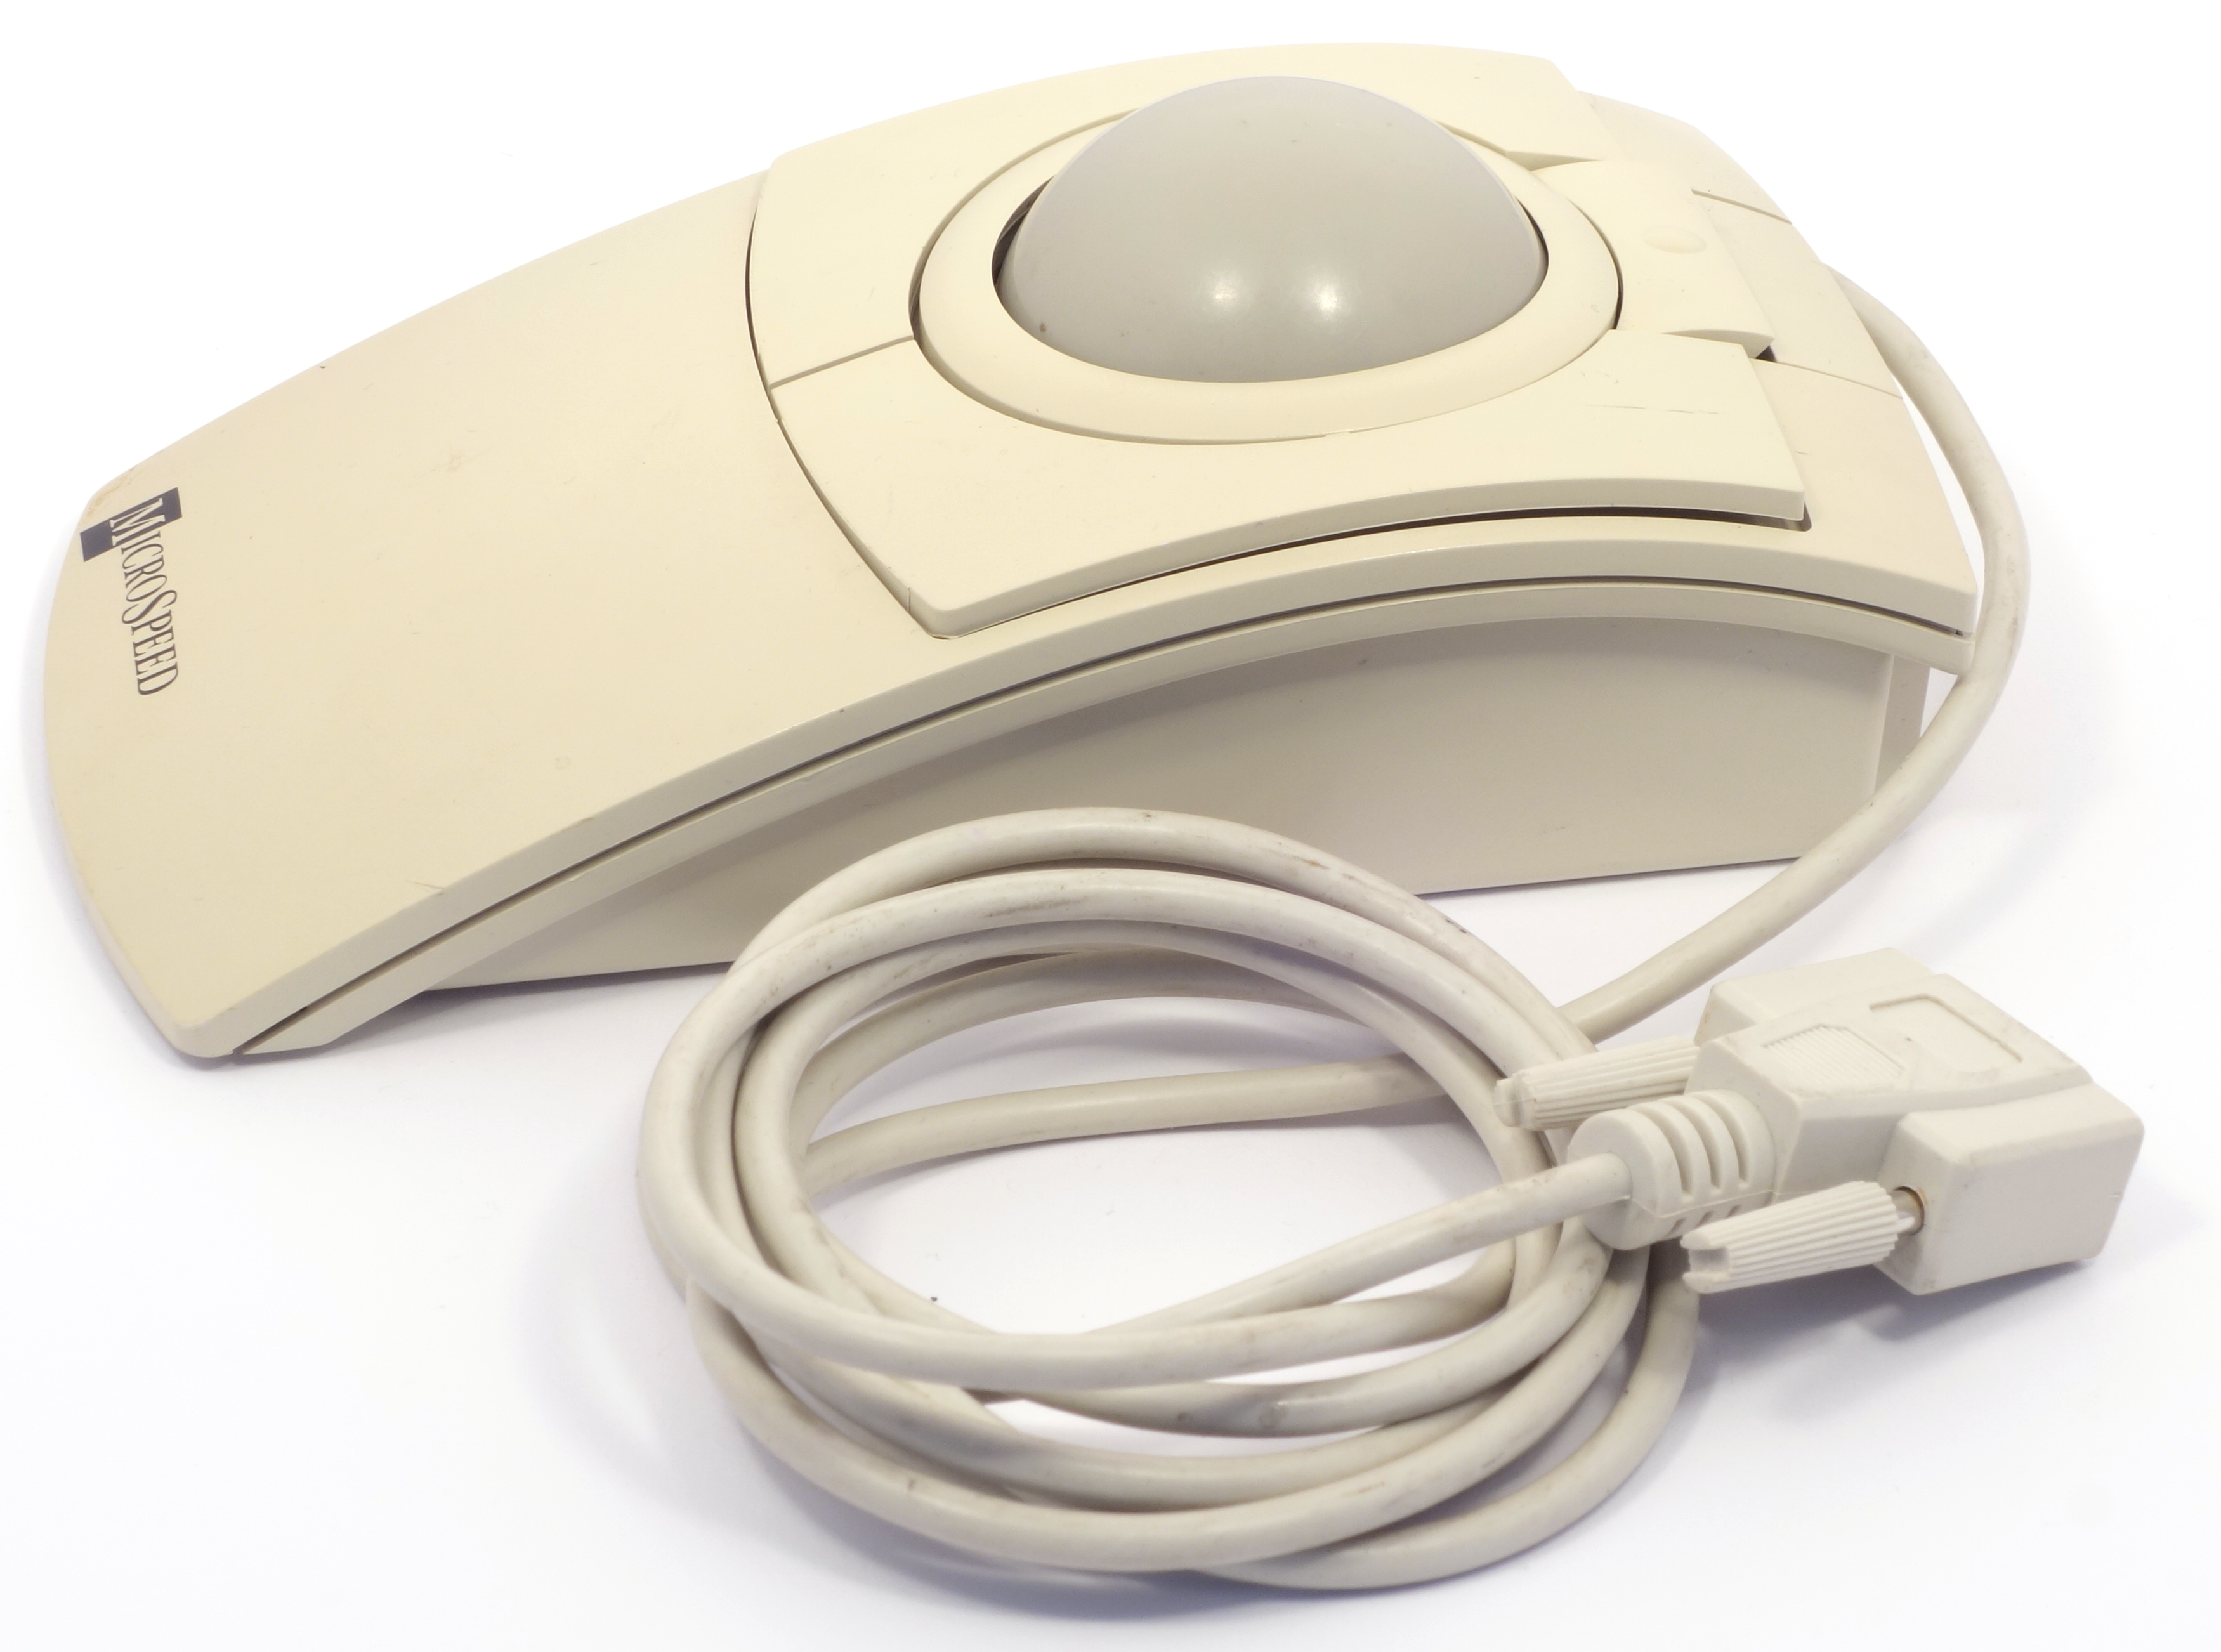
\includegraphics[scale=0.4]{1991_microspeed_pc-track/pic_30.jpg}
    \caption{MicroSpeed PC-TRACK trackball}
    \label{fig:PCTRACKPic}
\end{figure}

This trackball has a symmetrical design, suitable for both right- and left-handers (figure \ref{fig:PCTRACKTopBottom}). 

\begin{figure}[h]
    \centering
    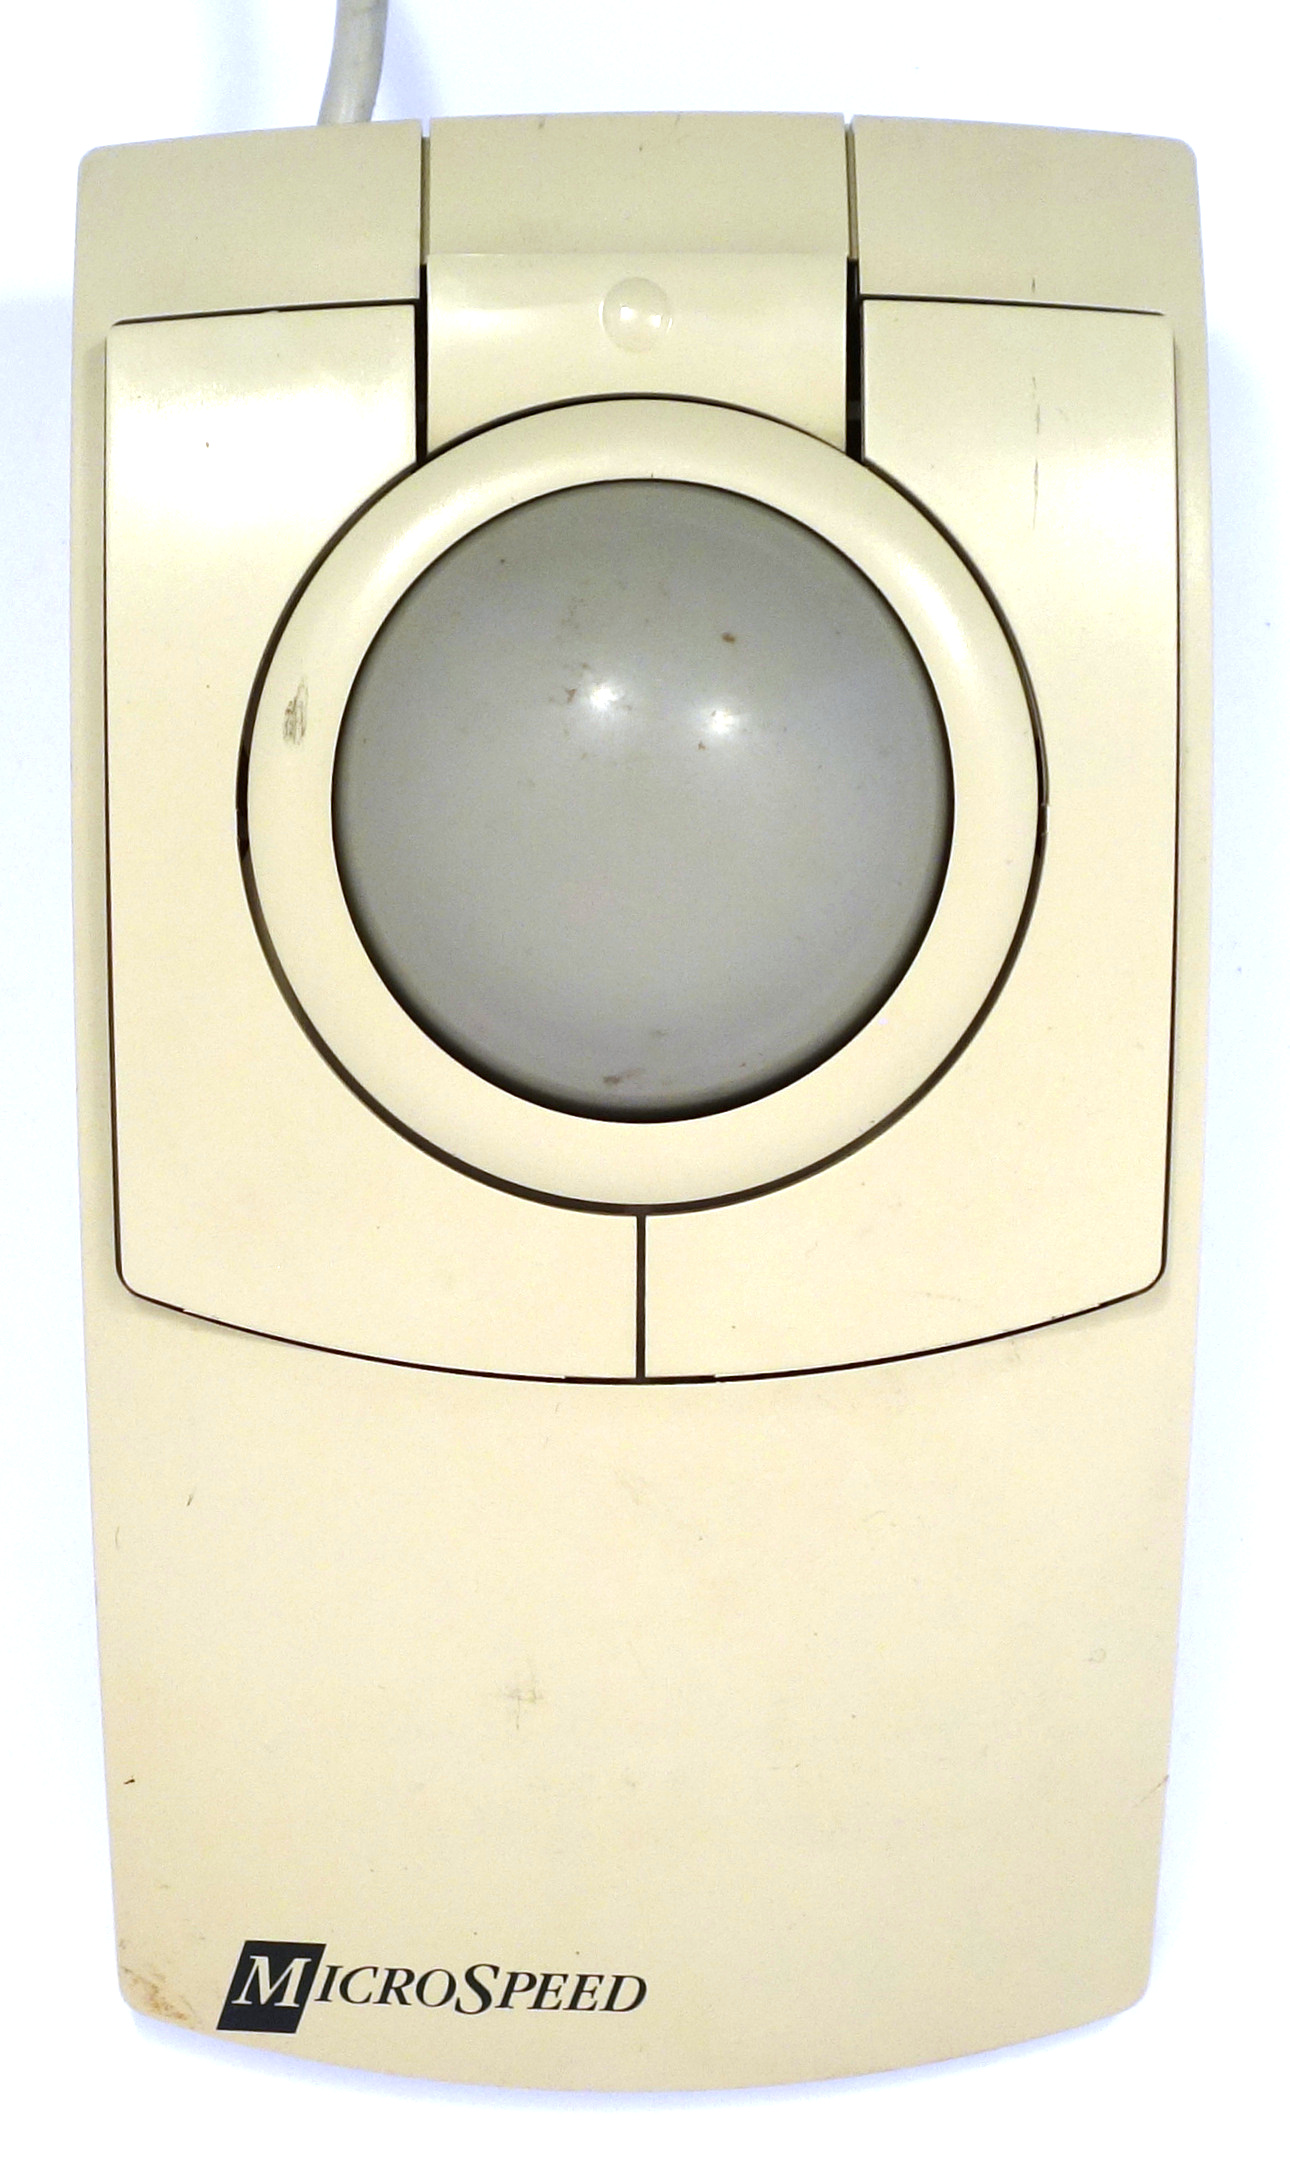
\includegraphics[scale=0.45]{1991_microspeed_pc-track/top_60.jpg}
    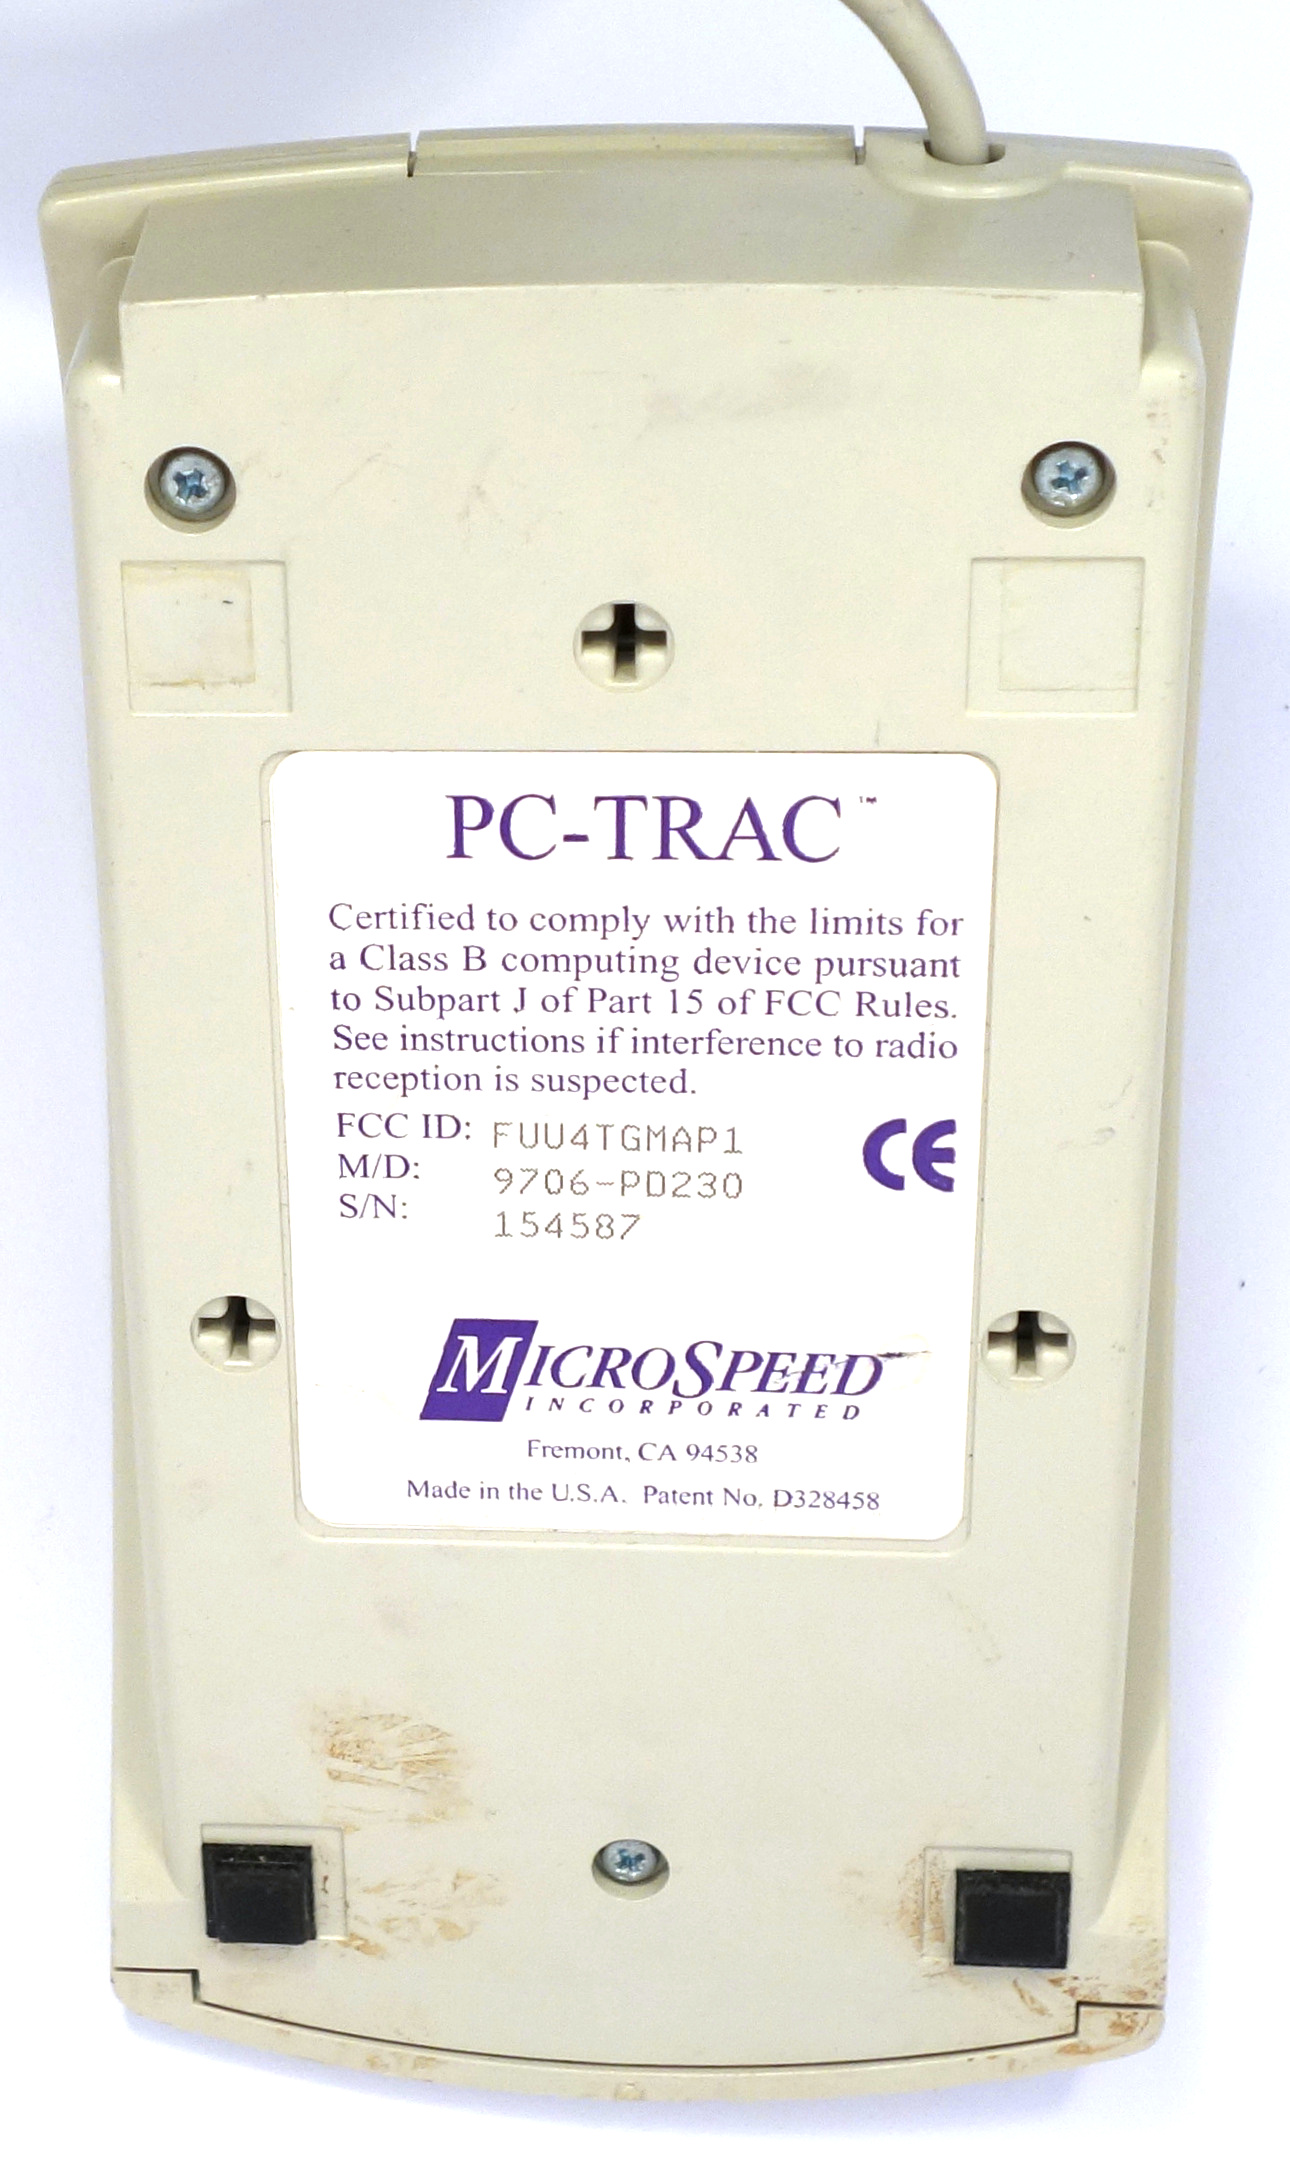
\includegraphics[scale=0.45]{1991_microspeed_pc-track/bottom_60.jpg}
    \caption{Fellowes Trackball, top and bottom views}
    \label{fig:PCTRACKTopBottom}
\end{figure}

The trackball is big (figure \ref{fig:PCTRACKSize}). MicroSpeed chose a 2.25-inch ball for this device because their research showed a significant increase in cursor positioning accuracy with a larger ball. Studies have also shown that greater ball weight also contributes to better accuracy; therefore this 2.25" ball has 30 percent more weight than the 2" ball and 70 percent more than the 1.5" ball used in other models.

\begin{figure}[h]
    \centering
    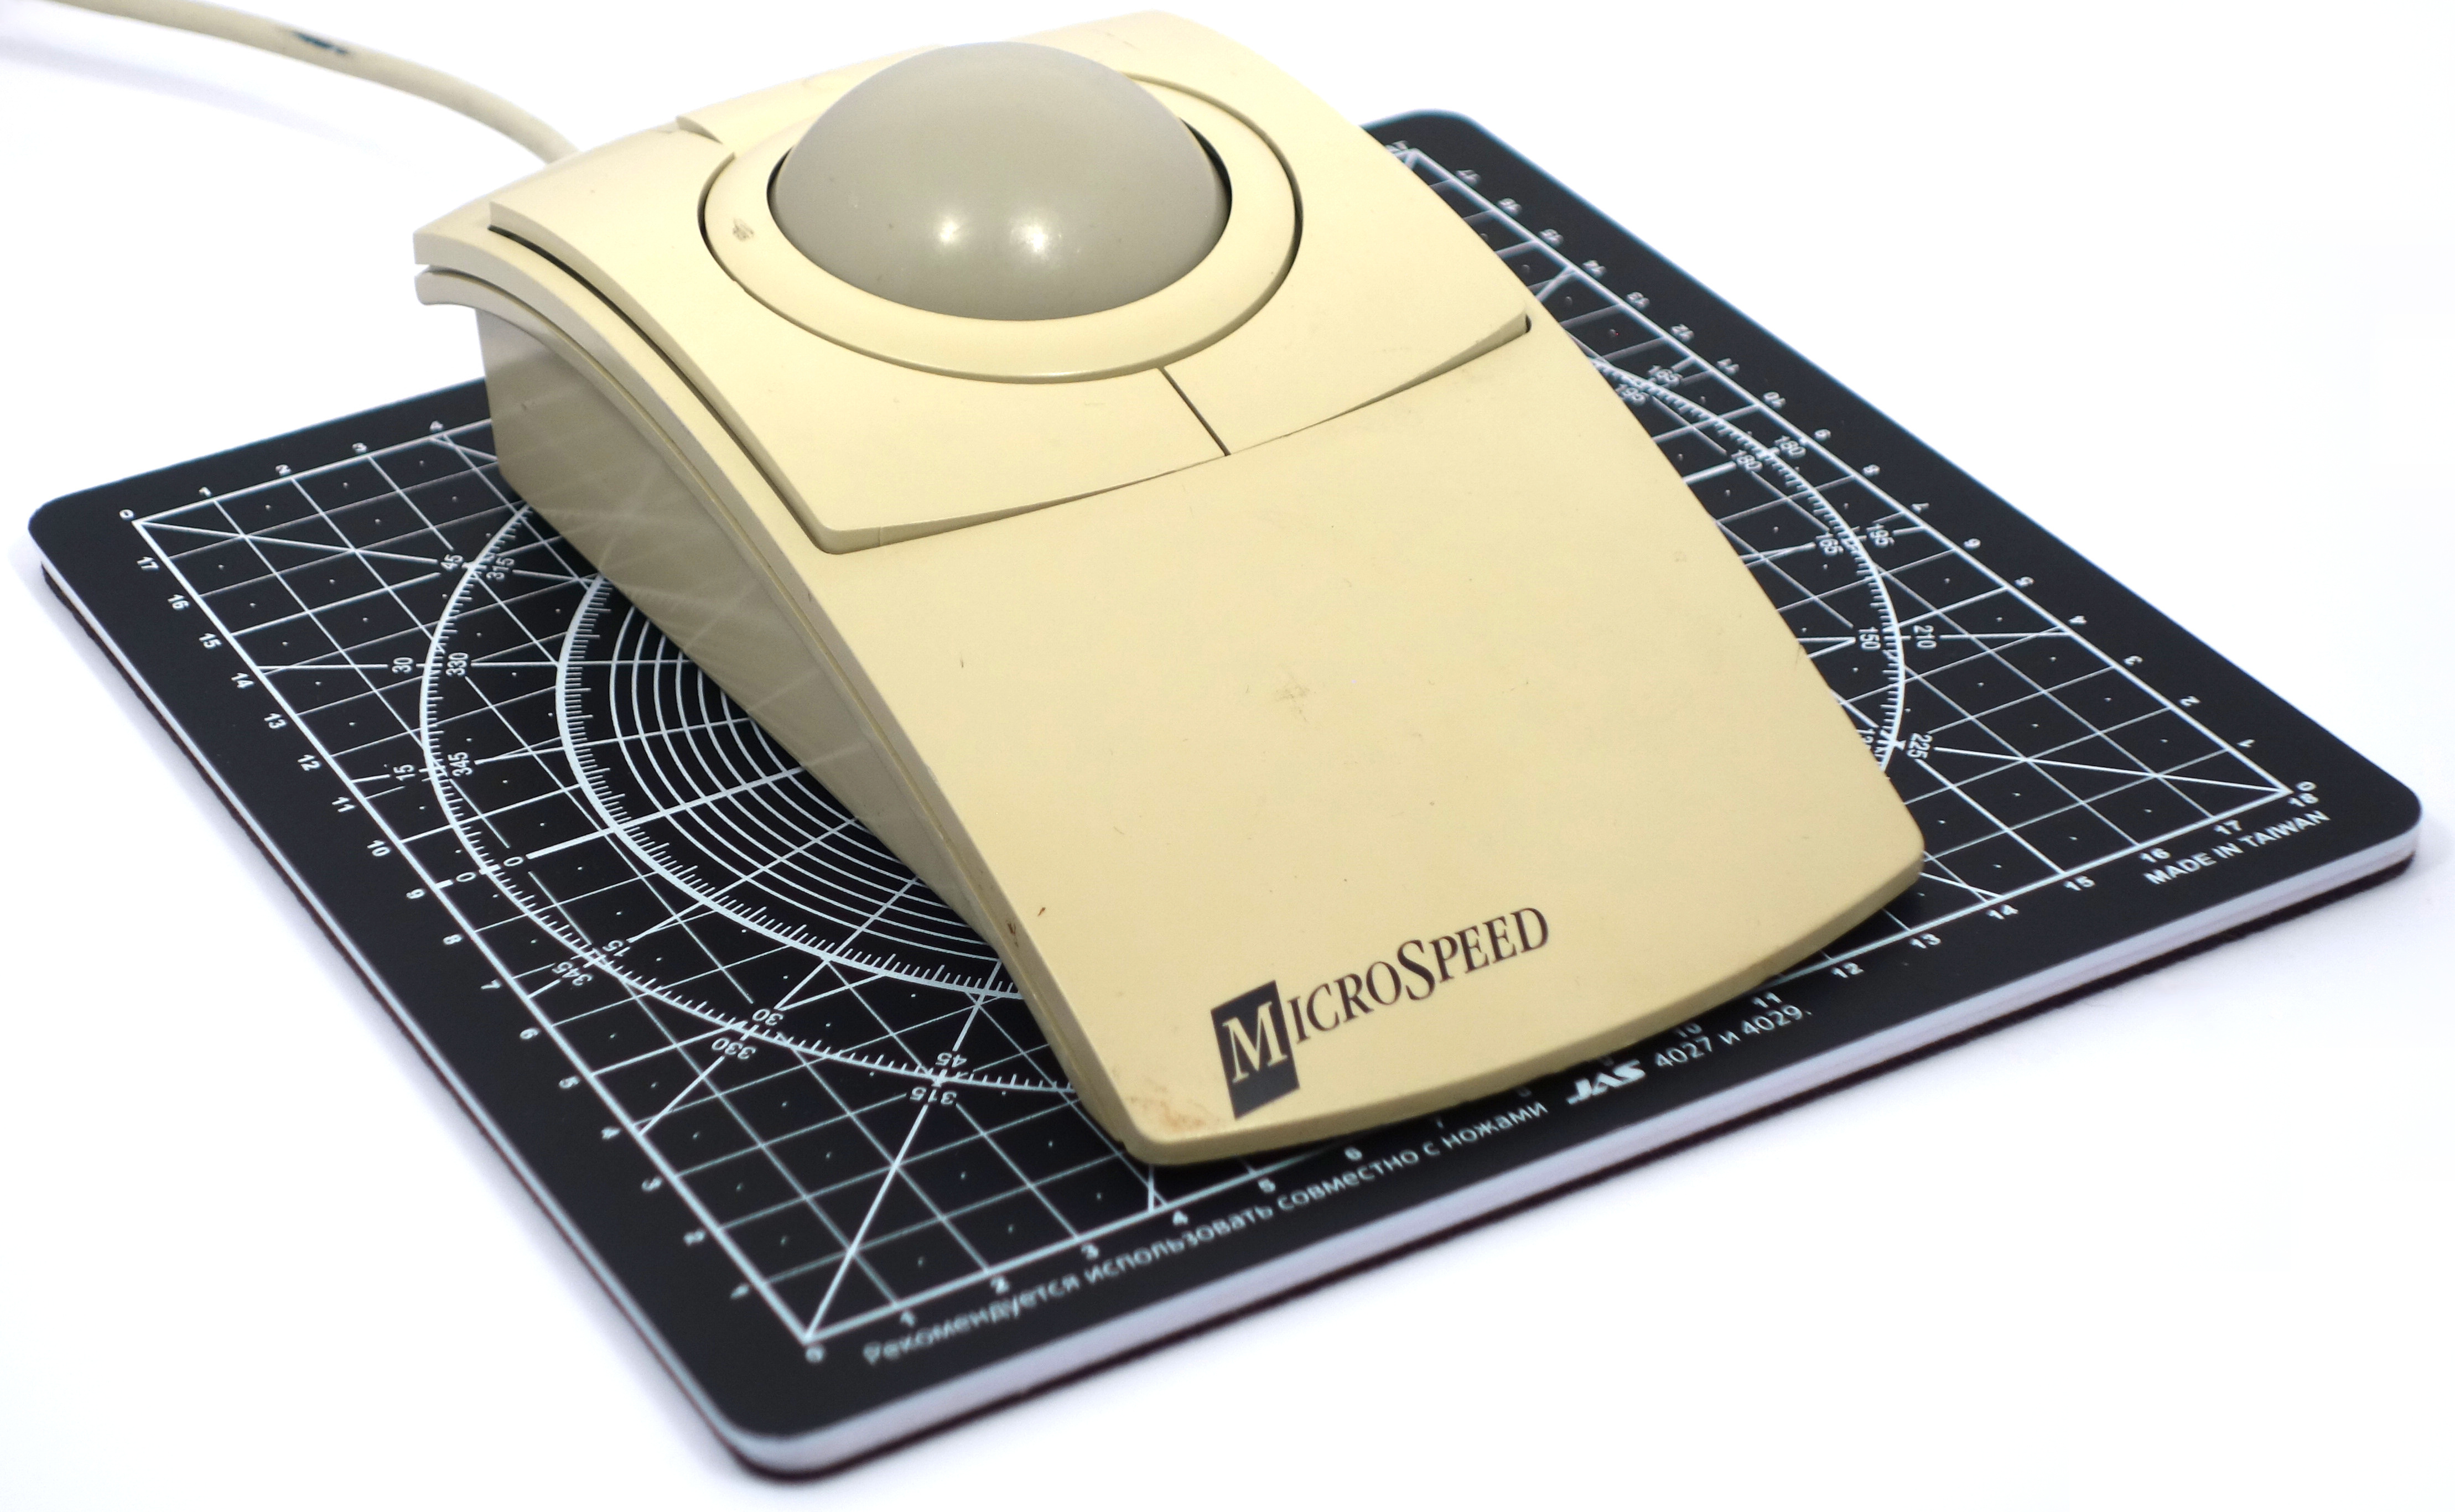
\includegraphics[scale=0.3]{1991_microspeed_pc-track/size_60.jpg}
    \caption{PC-TRACK on a graduated pad with a grid step of 1~cm}
    \label{fig:PCTRACKSize}
\end{figure}

On the sides, the ball is wrapped around by large convex buttons, and also there is an additional third button of a smaller size behind the ball. This arrangement of the main buttons is very convenient for the trackball; since the left and right buttons have a large area, the user can move the ball with the palm or fingertips, and use the thumb and little finger to press the buttons. In addition, this placement is symmetrical, so as mentioned in the beginning it works equally well for right-handers and left-handers \ref{fig:PCTRACKHand}. The PC-TRAC convex shape is designed to conform to the natural curve of the hand. The part of the case closest to the user actually merges with the table, and this, according to the manufacturer, eliminates the step present in earlier designs, thereby reducing the load on the wrist \cite{PC}.

\begin{figure}[h]
    \centering
    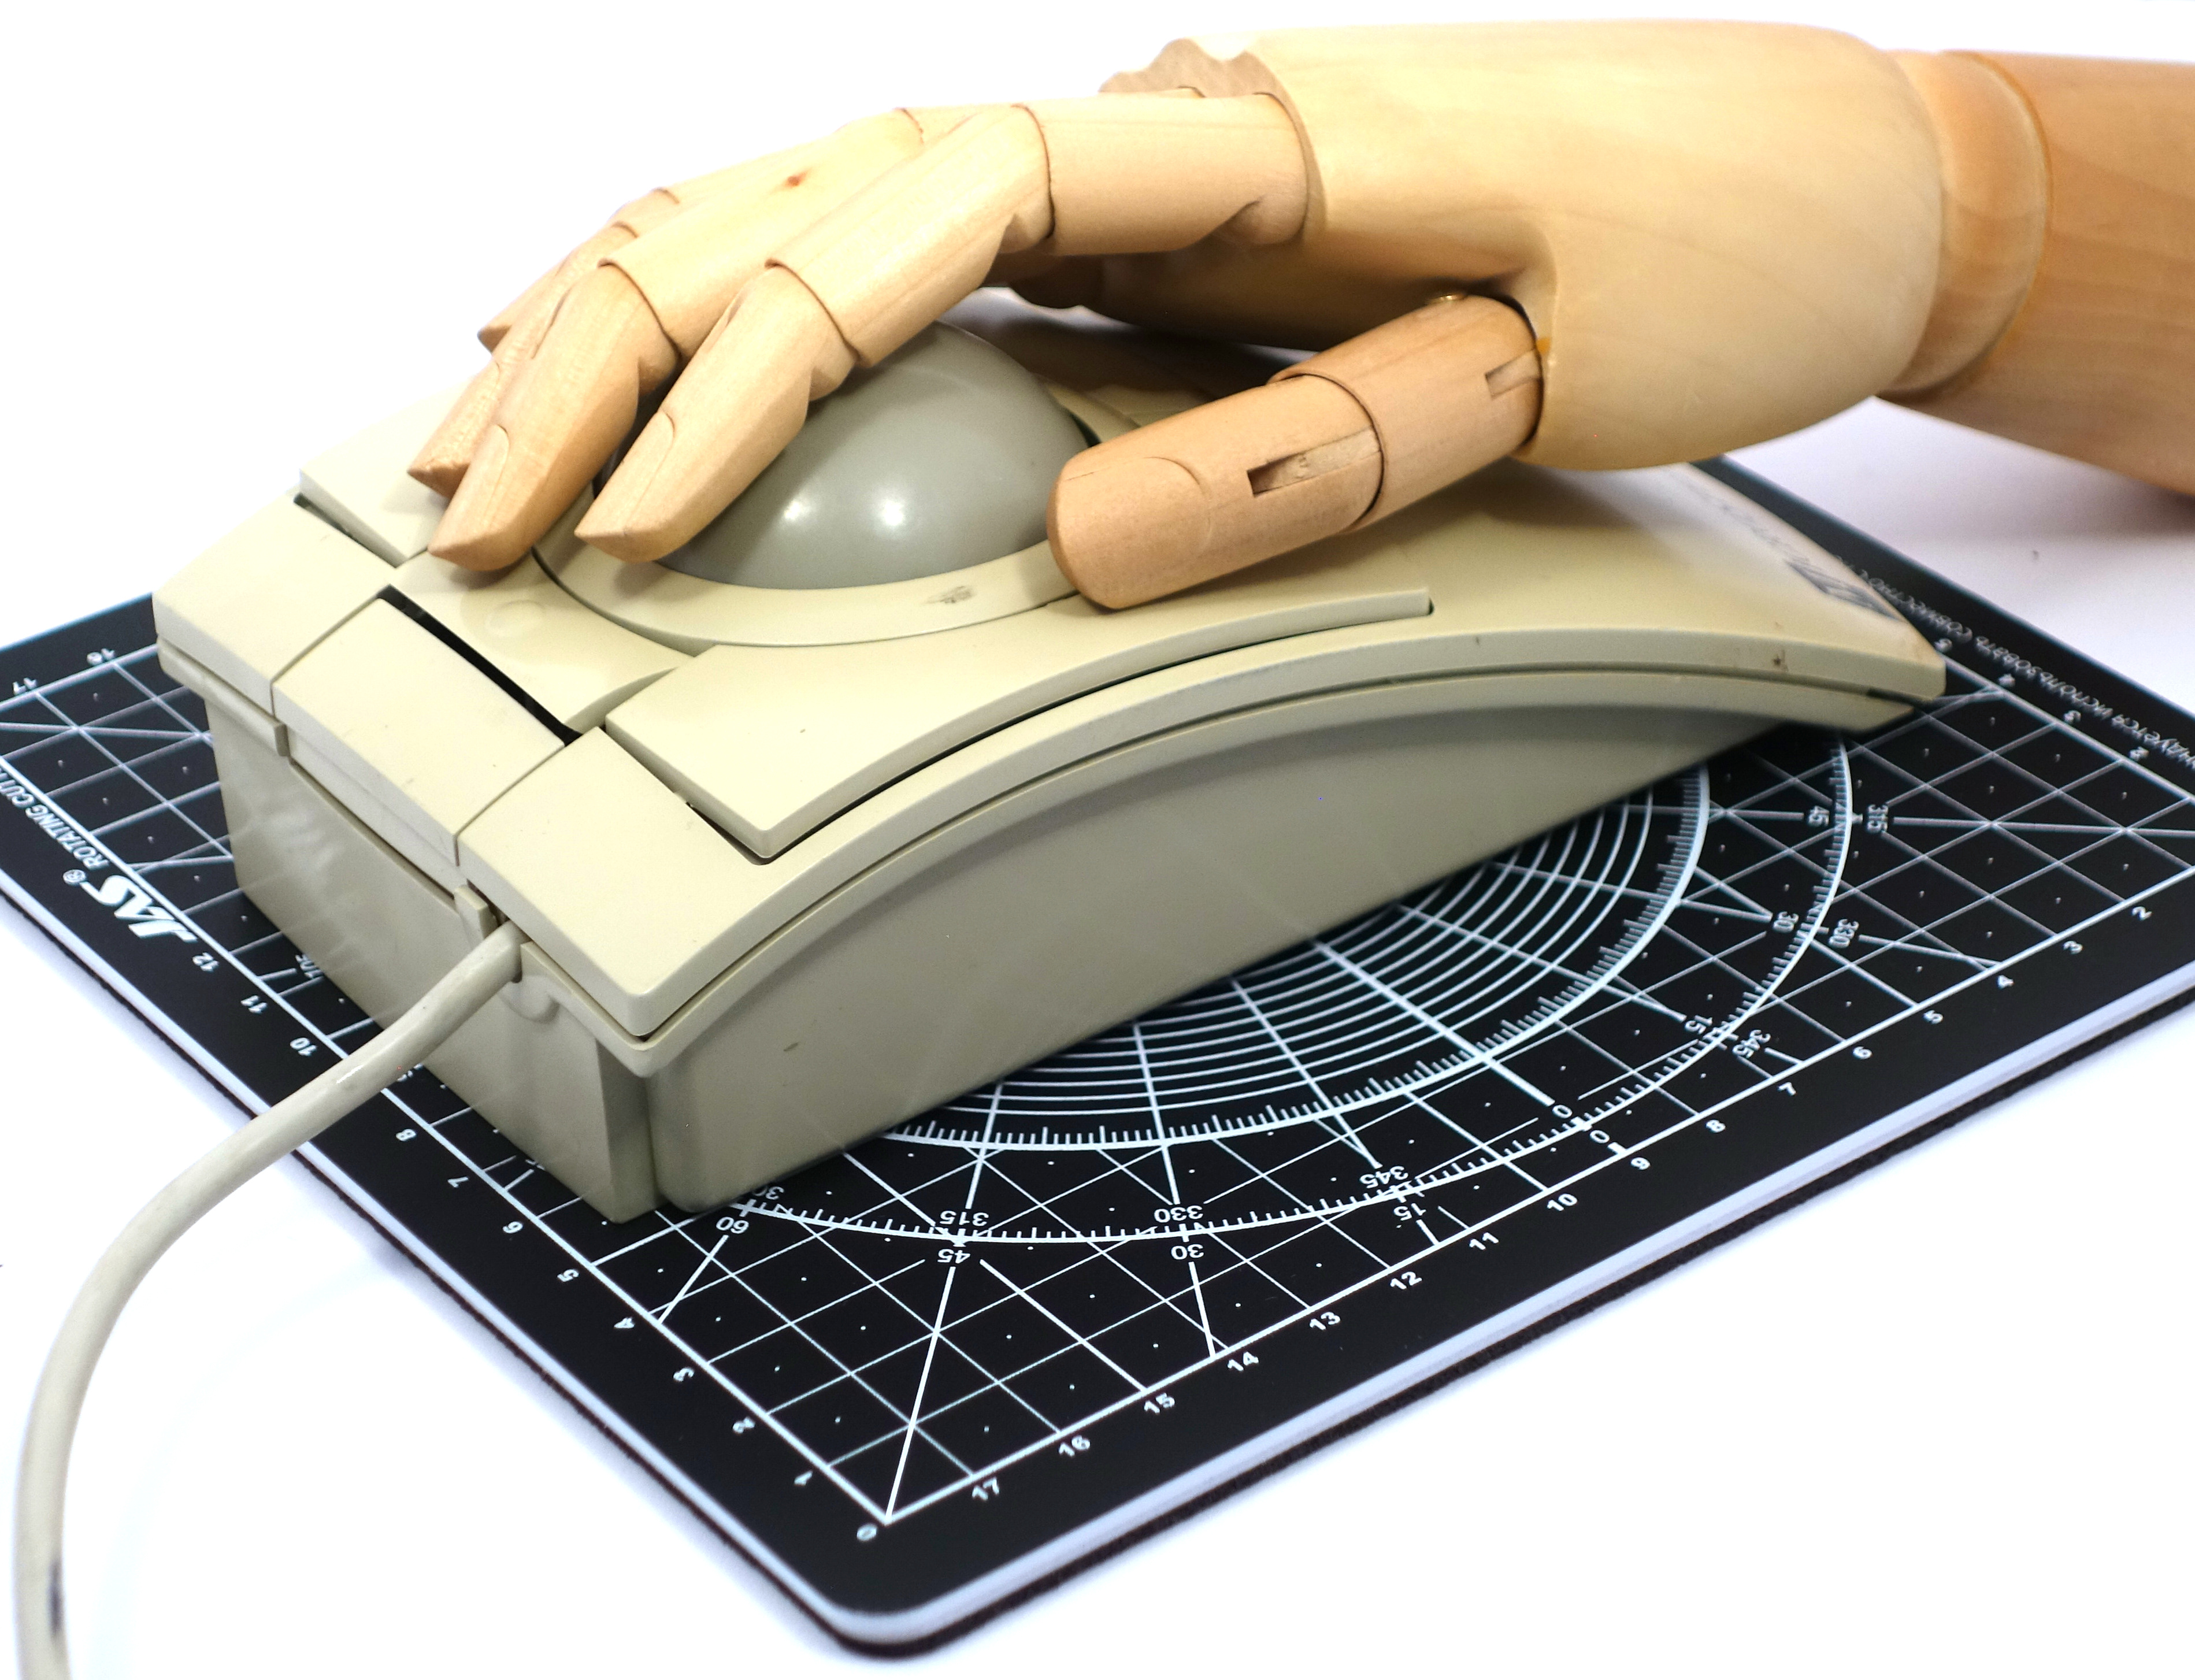
\includegraphics[scale=0.3]{1991_microspeed_pc-track/hand_60.jpg}
    \caption{PC-TRACK with a human hand model}
    \label{fig:PCTRACKHand}
\end{figure}

The smaller third button can be used as the middle mouse button or as a drag lock. One of the main problems with using trackballs in graphical interfaces such as Windows at the turn of the 80s and 90s was that it was difficult for the user to move the pointer while holding down the button. If the drag-and-drop feature is enabled, you can press the middle button after the pointer is positioned at the start position, move the pointer to the end position, and press the middle button again to finish dragging the object (from the computer's point of view, the user kept the button pressed the whole time). In addition to this feature, PC-TRAC also has a chord mode that allows you to simulate holding both buttons while moving the mouse.

In terms of software, the trackball is fully compatible with the Microsoft mouse driver. It came with PrecisionPointer drivers for DOS and Windows that offer a number of trackball-specific improvements, such as acceleration when the cursor moves (the distance the pointer moves depends on how fast you spin the ball). The kit also includes a key remapping utility, a driver for console applications that simulates the operation of cursor keys when the ball rotates, as well as a separate driver for playing Tetris.

\begin{figure}[h]
    \centering
    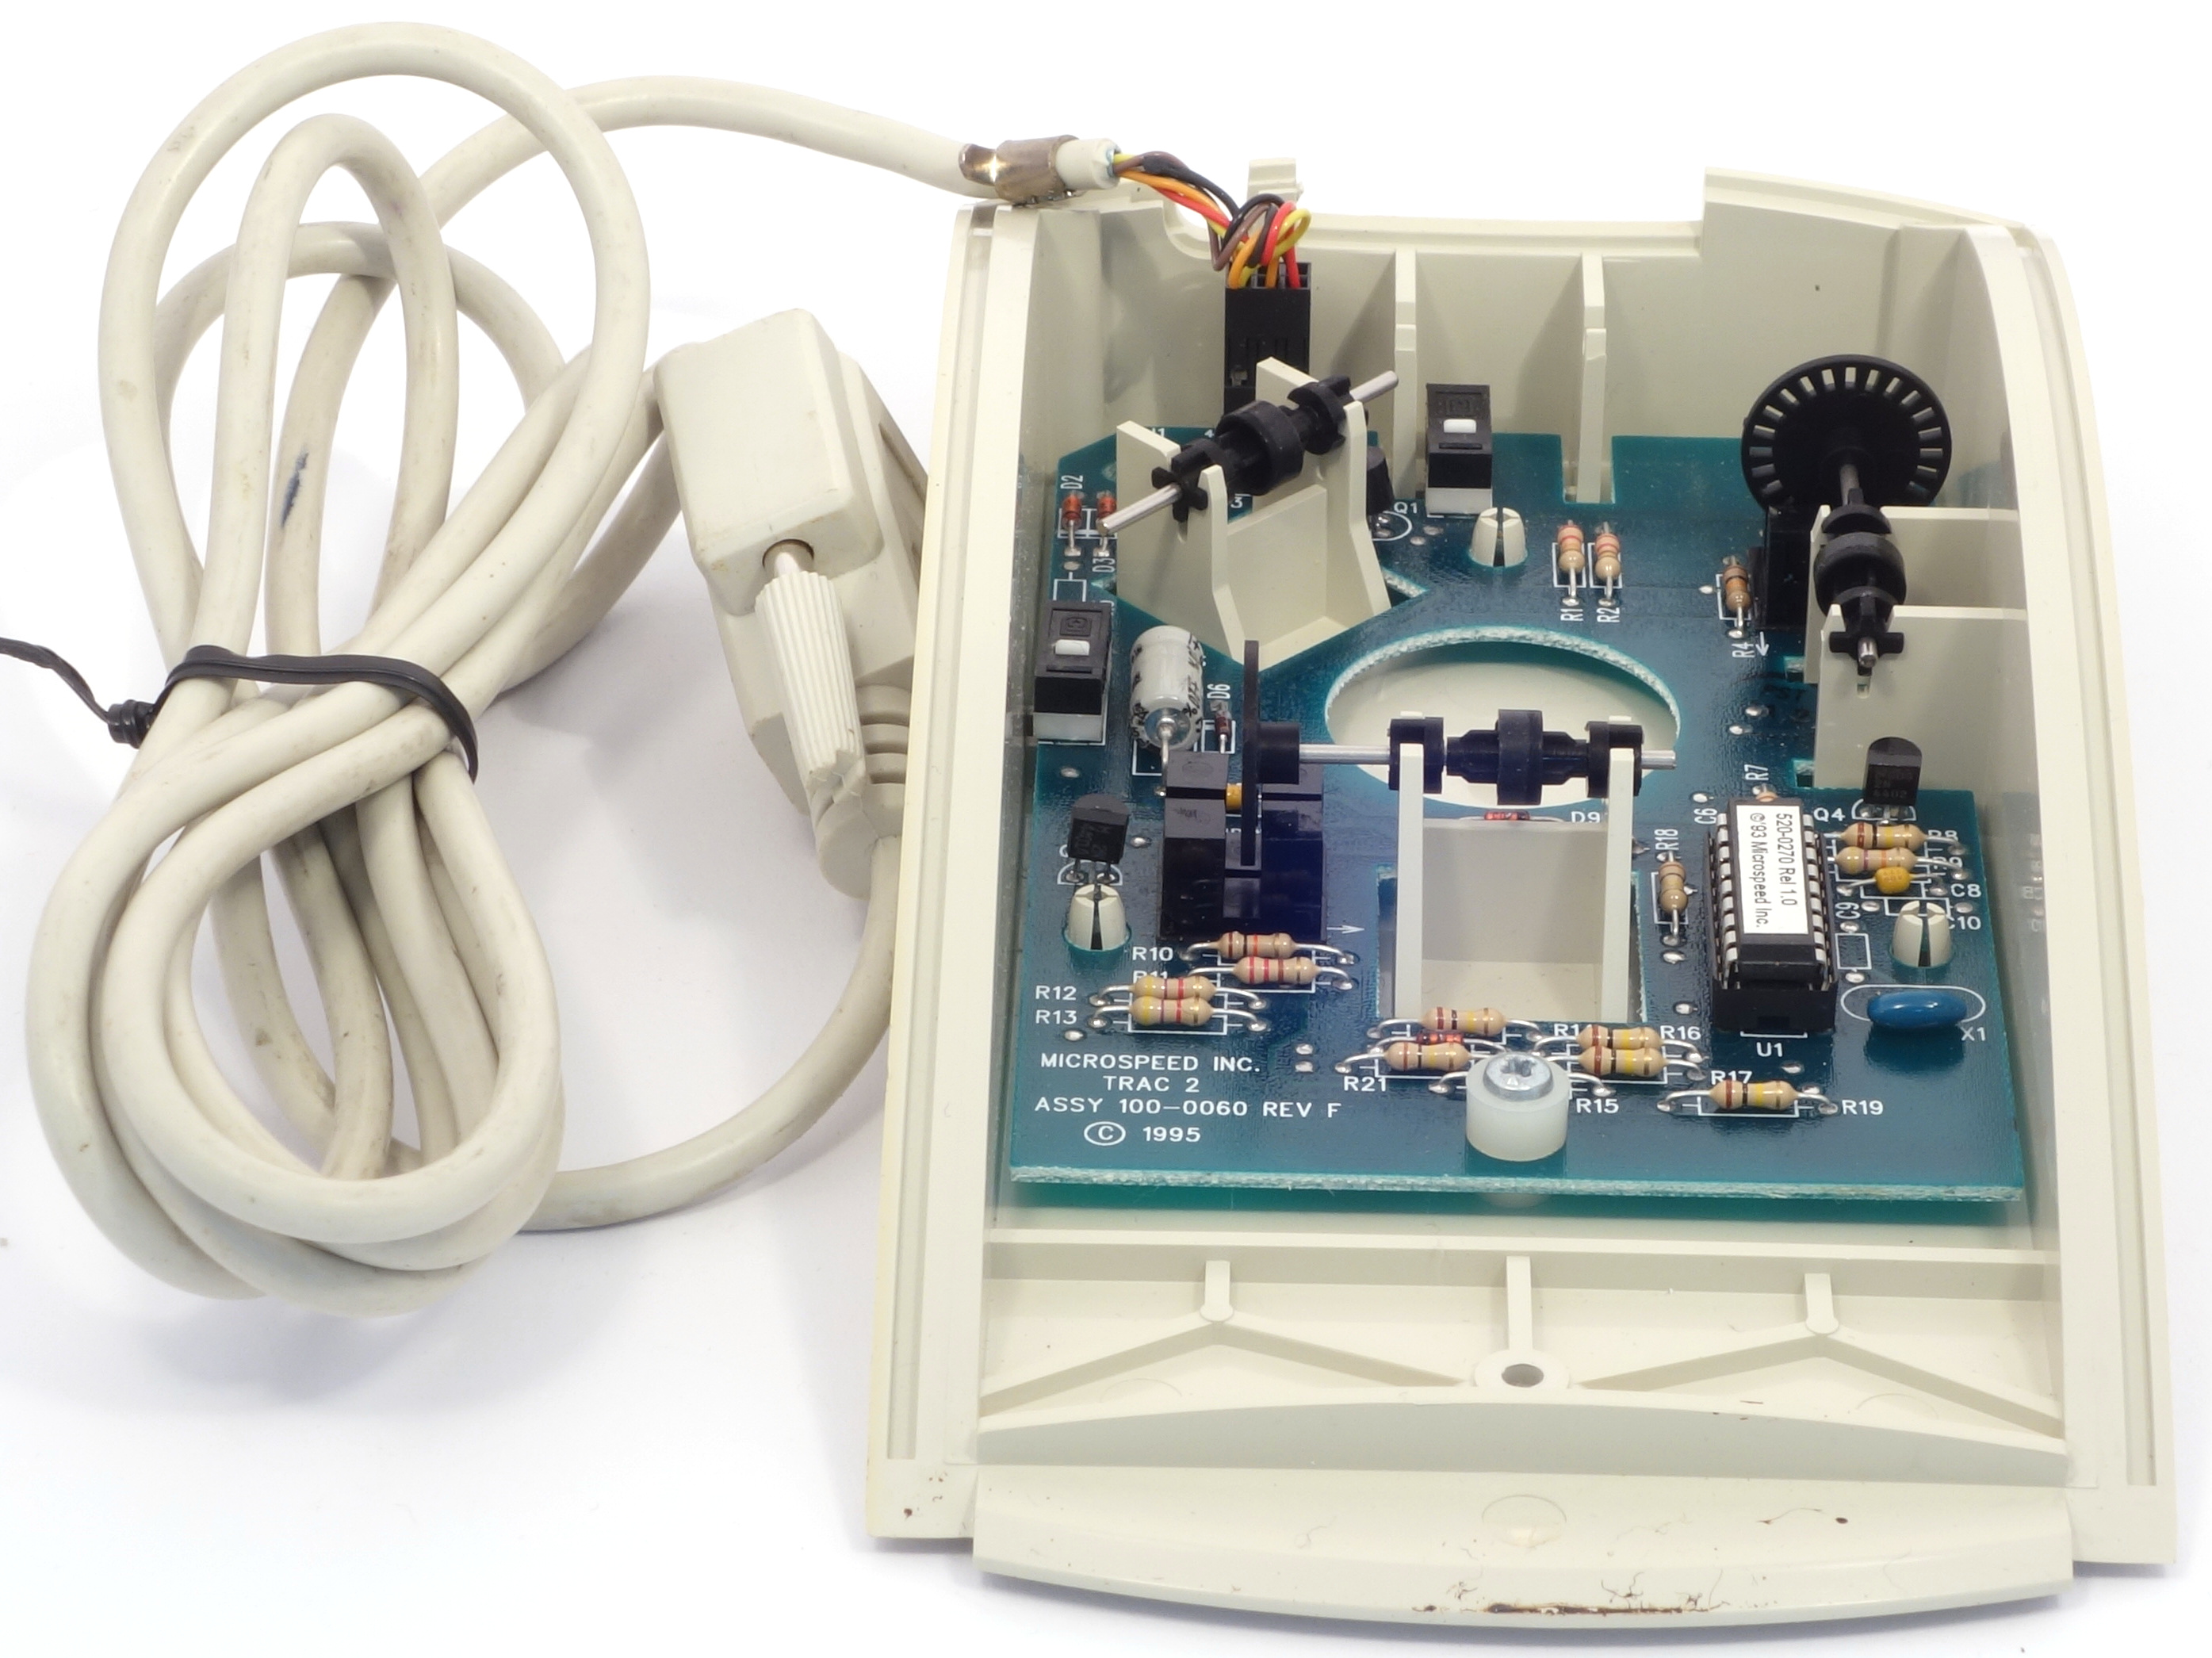
\includegraphics[scale=0.7]{1991_microspeed_pc-track/inside_30.jpg}
    \caption{PC-TRACK disassembled}
    \label{fig:PCTRACKInside}
    \end{figure}

Trackball internals are shown on figure \ref{fig:PCTRACKInside}. As you can see, PC-TRACK trackball follows the traditional opto-mechanical scheme. MicroSpeed have used rollers with rolling bearings made of the Delrin plastic. Advertising noted that in addition to the fact that they are self-lubricating, they are also more resistant to the formation of caverns, pollution and damage from mechanical shocks (for example, when falling down) than metal bearings.

\begin{thebibliography}{9}
\bibitem {PC} MiCROSPEED PC-TRACK // Compute! Magazin,  Iss. 132, August 1991. - p. 50. \url{https://archive.org/details/1991-08-compute-magazine/page/n51/mode/2up}
\end{thebibliography}
\end{document}
